\documentclass[11pt,a4paper]{article}
\usepackage[margin=2.2cm]{geometry}
\usepackage{fontspec}
\usepackage{xeCJK}
\usepackage{graphicx}
\usepackage{booktabs}
\usepackage{array}
\usepackage{float}
\usepackage{caption}
\usepackage{amsmath}
\usepackage[hidelinks]{hyperref}

\setmainfont{Times New Roman}
\setCJKmainfont{Songti SC}
\linespread{1.12}
\captionsetup{font=small,labelfont=bf}
\renewcommand{\arraystretch}{1.16}

\title{\textbf{Bitcoin Trading Bot Optimisation with WOA and PSO}}
\author{}
\date{}

\begin{document}
\maketitle

\begin{abstract}
This project designs and optimizes a Bitcoin trading bot based on weighted moving average (WMA) crossovers. It primarily compares the Whale Optimization Algorithm (WOA) and Particle Swarm Optimization (PSO), using Random Search and Buy-and-Hold as baselines. The report addresses three key questions: the performance differences among various search methods under the same fitness evaluation budget; the relationship between SMA, LMA, and EMA weights and window parameters and strategy performance in a 14-dimensional composite bot; and the trade-offs between search space complexity, generalization, and computational cost between a 2-dimensional simple bot and a 14-dimensional composite bot. The results show that WOA and PSO can significantly improve training set fitness, but neither consistently outperforms Buy-and-Hold on the test set; Random Search achieved the highest single-test result, reminding us that historical backtesting optimization carries significant generalization risks.
\end{abstract}

\section{Introduction}
The objective of this experiment is to design an AI trading bot using nature-inspired optimization algorithms and to evaluate its training performance and unseen test performance on the Bitcoin Historical Dataset. The trading rules are based on moving average crossover signals from technical analysis, and the optimization algorithm must search the parameter space for a set of bots capable of generating high backtest returns. This report analyzes algorithm performance, signal parameter interpretation, and search space complexity within a unified framework.

This report focuses on three key questions. First, given the same fitness evaluation budget, how do the optimization performance and generalization capabilities of WOA, PSO, and the Random Search baseline differ? Second, how do the weight combinations of SMA, LMA, and EMA, along with window lengths, in a 14-dimensional composite bot influence the structure of trading signals, and what is the relationship between these factors and the final train/test performance? Third, how do the differences in search space complexity between the 2-dimensional Simple Bot and the 14-dimensional composite Bot affect the trade-off between optimization effectiveness, generalization performance, and computational cost?

\section{Bot Design and Parameterisation}

The bot’s core trading logic is based on moving average crossovers: it buys when the more sensitive HIGH signal crosses above the smoother LOW signal, and sells when the HIGH signal falls below the LOW signal.
All trades follow these rules: Initial capital is 1,000 USD; when buying, use all available cash to purchase BTC; when selling, sell all BTC; a 3\% fee is deducted from each trade; if BTC is still held at the end of the sequence, it is forcibly sold at the last price.

The 14-dimensional composite bot uses SMA, LMA, and EMA to construct the two signal lines, HIGH and LOW:
\begin{equation}
HIGH=\frac{w_1SMA(d_1)+w_2LMA(d_2)+w_3EMA(d_3,\alpha_1)}{w_1+w_2+w_3},
\end{equation}
\begin{equation}
LOW=\frac{w_4SMA(d_4)+w_5LMA(d_5)+w_6EMA(d_6,\alpha_2)}{w_4+w_5+w_6}.
\end{equation}
The parameter vector is
\[
x=[w_1,w_2,w_3,d_1,d_2,d_3,\alpha_1,w_4,w_5,w_6,d_4,d_5,d_6,\alpha_2].
\]
The weight range is $[0,1]$; the HIGH window range is $[2,50]$; the LOW window range is $[2,100]$; and the $\alpha$ range for the EMA is $[0.01,0.99]$. Window parameters are rounded to the nearest integer when used. To analyze the search space complexity, a 2-dimensional Simple Bot was also implemented, optimizing only the short-term SMA window $N_1\in[2,50]$ and the long-term SMA window $N_2\in[10,200]$.


\section{Algorithms and Experimental Design}

WOA is based on Mirjalili and Lewis \cite{mirjalili2016} and updates candidate solutions through three behaviors: enveloping the current optimal solution, spiral updates, and random search. The control parameter $a$ linearly decreases from 2 to 0, causing the algorithm to favor exploration in the early stages and exploitation in the later stages. PSO is based on the work of Kennedy and Eberhart \cite{kennedy1995}, where particle velocities are driven jointly by the individual’s historical best $pbest$ and the population’s best $gbest$. This project implements the version without inertial weights and uses $V_{max}$ to limit the velocity in each dimension. Random Search uses uniform random sampling; it is not used as a primary optimization algorithm but rather to determine whether complex search methods are truly superior to simple sampling.


The Genetic Algorithm (GA) was not retained as an implementation algorithm in the final system. The primary reason is that GA is better suited for broad exploration at the levels of coding structure, combinatorial selection, or rule-based frameworks; however, this project has a fixed bot structure, and the core task is to optimize continuous weights, window length, and EMA $\alpha$ within a defined search space. Therefore, WOA and PSO are more directly suited to this parameter optimization problem.

The data used is the daily closing price of BTC from the Bitcoin Historical Dataset \cite{btc_dataset}. The training set covers the period from November 28, 2014, to December 31, 2019, totaling 1,860 days; the test set covers the period from January 1, 2020, to March 1, 2022, totaling 791 days. The optimization process uses only the training set; the test set is used solely for final evaluation. WOA, PSO, and Random Search use the same 5 seeds (42, 123, 456, 789, 1024) and 5,000 fitness evaluations in the 14-dimensional main experiment. The 2-dimensional control experiment compares only WOA and PSO. The PSO sensitivity analysis compares performance for population sizes of 20, 50, and 100, while keeping the total evaluation budget constant.

\section{Results and Analysis}

\subsection{Focus Question 1: Algorithm Performance Under the Same Budget}

Figure \ref{fig:convergence} shows the convergence curves for the training set in the 14-dimensional main experiment. The average training fitness for WOA was 43,158.94 USD, for PSO it was 40,516.05 USD, and for Random Search it was 33,344.62 USD. Under the same evaluation budget, both WOA and PSO were able to continuously improve the best-so-far fitness on the training set more effectively than Random Search, demonstrating that nature-inspired optimization can indeed leverage price patterns observed during the training phase.



\begin{figure}[H]
\centering
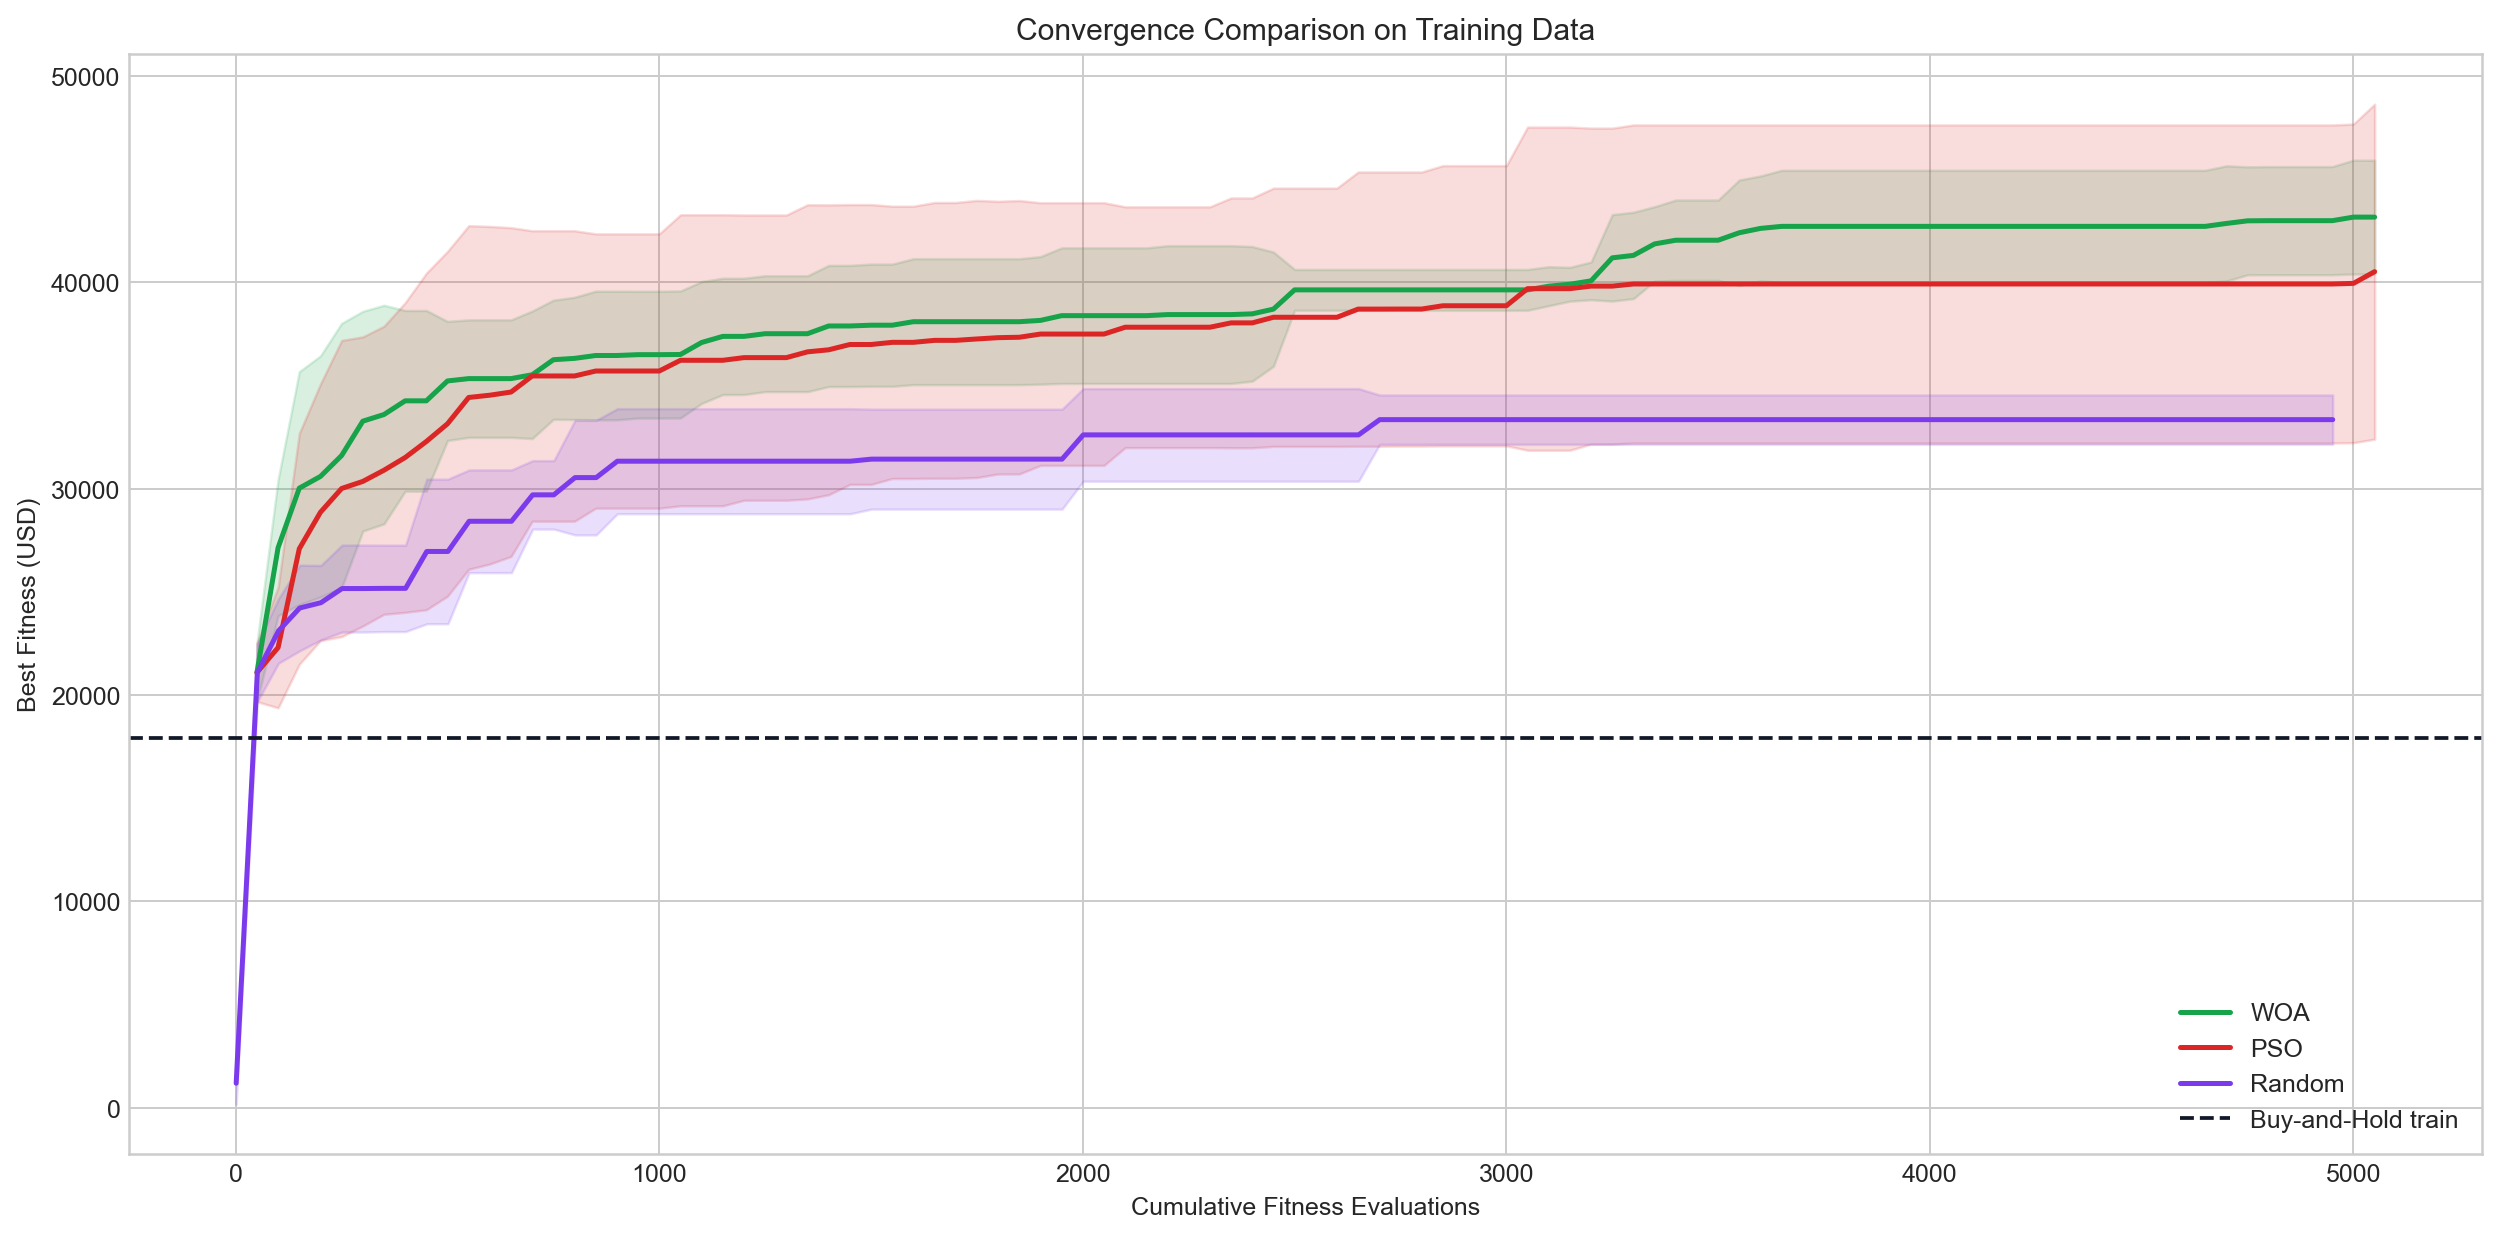
\includegraphics[width=0.92\linewidth]{outputs/figures/convergence_comparison.png}
\caption{Training convergence comparison under the same evaluation budget.}
\label{fig:convergence}
\end{figure}

\begin{table}[H]
\centering
\caption{Summary of key experimental results.}
\small
\begin{tabular}{llrrrr}
\toprule
Algorithm & Bot Type & Train Mean & Test Mean & Best Test & Time(s)\\
\midrule
WOA & 14D & 43158.94 & 4237.88 & 5862.44 & 1.1\\
PSO & 14D & 40516.05 & 3796.67 & 4099.03 & 1.2\\
Random & 14D & 33344.62 & 5358.84 & 7604.03 & 1.4\\
WOA & 2D & 40753.05 & 592.93 & 617.28 & 0.6\\
PSO & 2D & 40137.37 & 694.89 & 1005.34 & 0.6\\
Buy-and-Hold & Baseline & 17924.71 & 5660.26 & 5660.26 & 0.0\\
\bottomrule
\end{tabular}
\end{table}

The test set results changed the conclusion. WOA’s average test fitness was 4237.88 USD, higher than PSO’s 3796.67 USD, but both were lower than Buy-and-Hold’s 5660.26 USD. Random Search achieved an average test fitness of 5,358.84 USD, close to Buy-and-Hold, and recorded the highest single-test result of 7,604.03 USD. This does not imply that Random Search is systematically superior, but rather indicates that the fitness landscape for this problem is highly noisy, and the training-phase optimum may not generalize.

\begin{figure}[H]
\centering
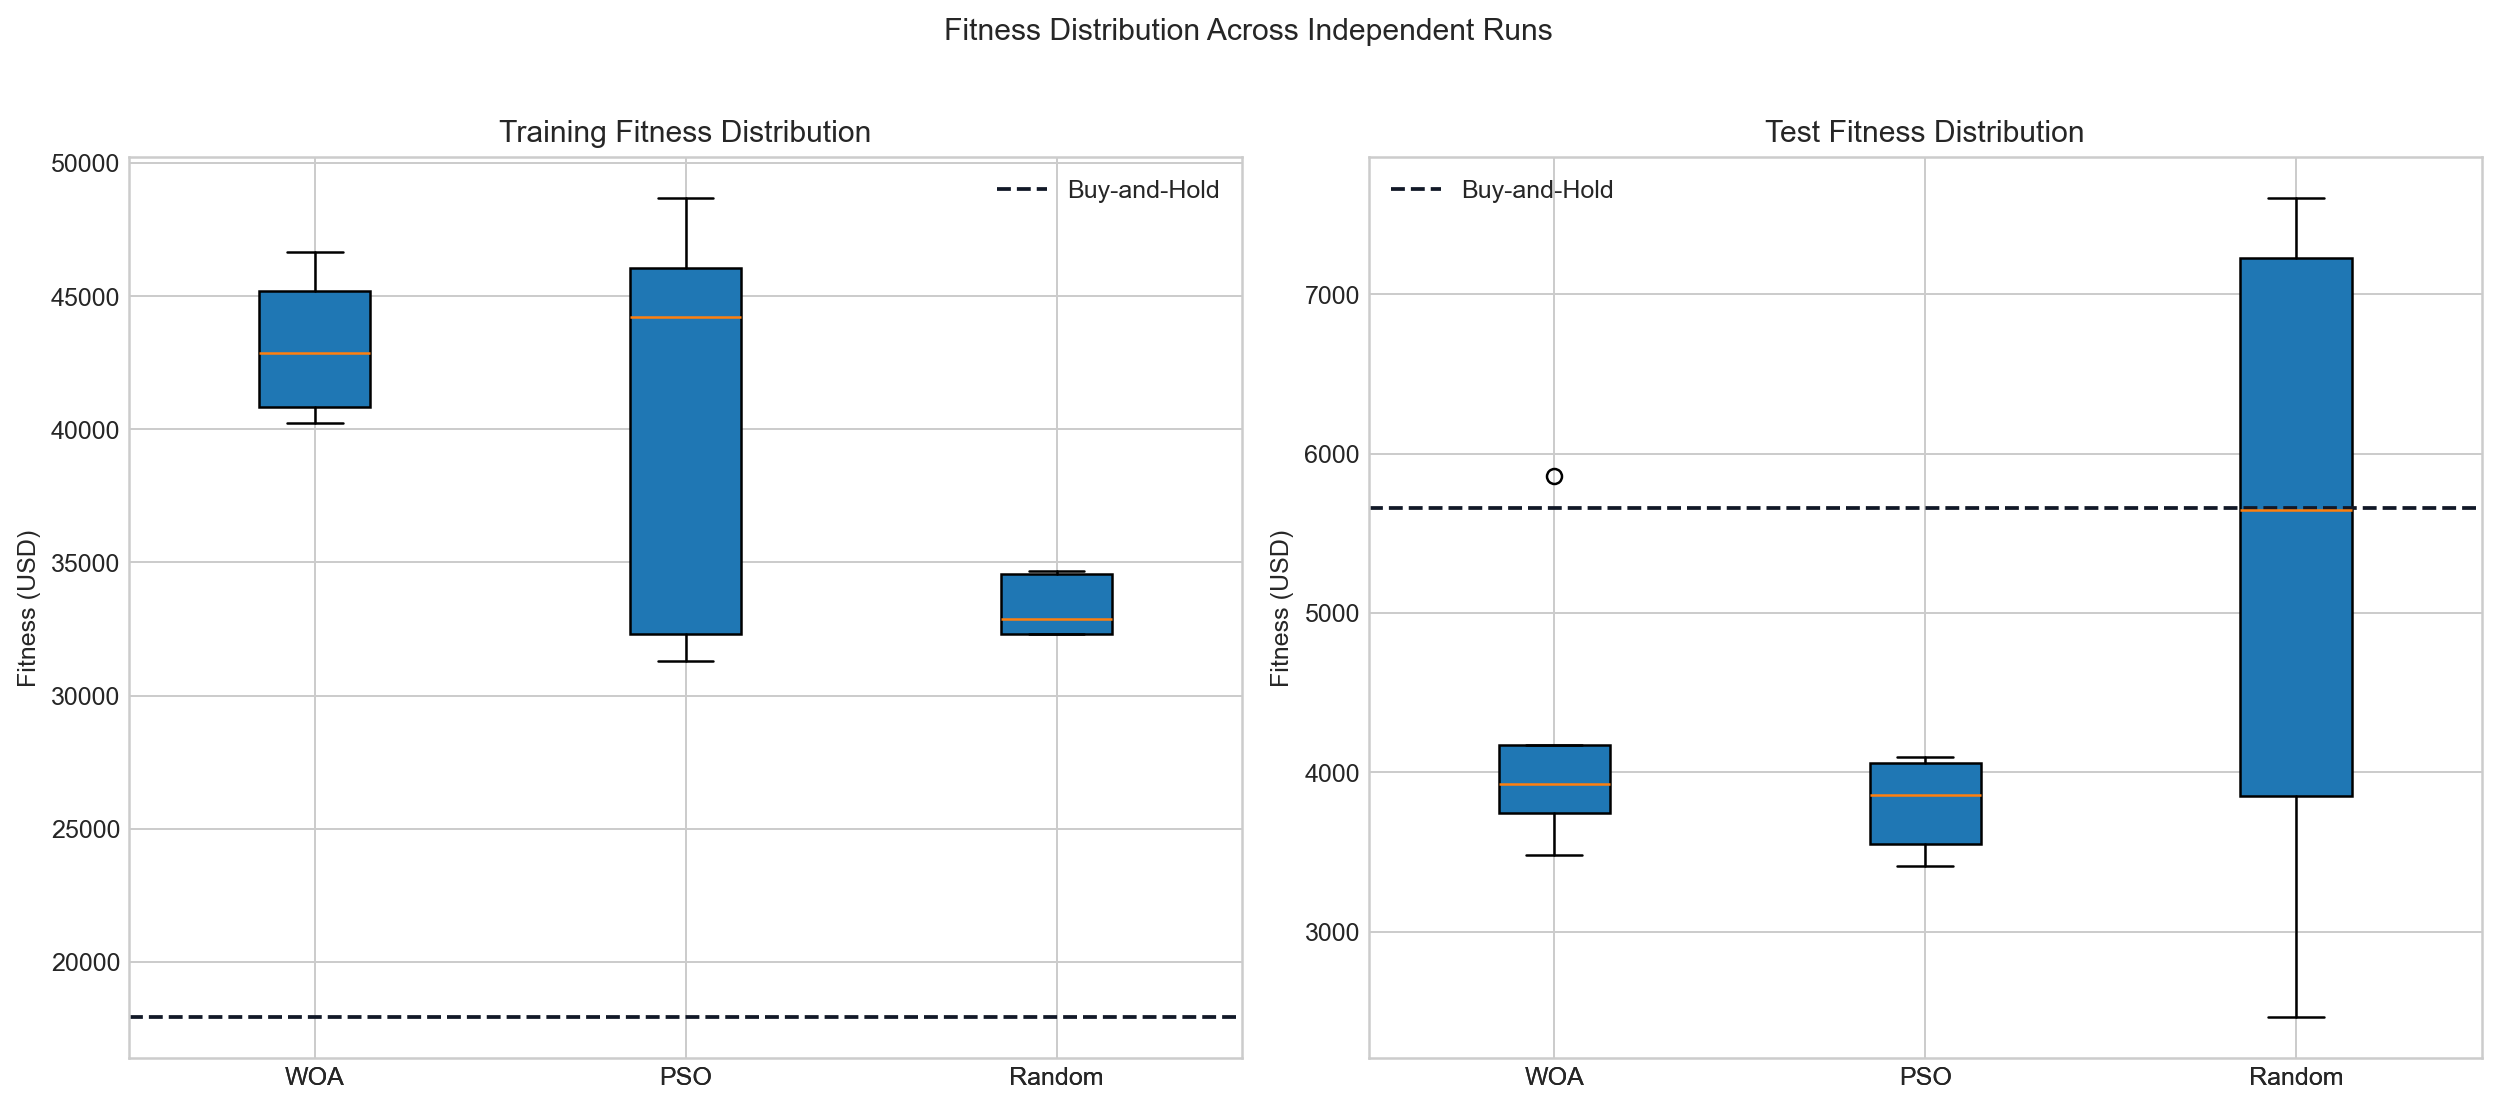
\includegraphics[width=0.92\linewidth]{outputs/figures/fitness_boxplots.png}
\caption{Train/test fitness distributions over five independent runs.}
\label{fig:box}
\end{figure}

Figure \ref{fig:trade} shows the trading details of the best test bot overall. This bot was generated via random search, executed only two trades, and achieved a test fitness of 7,604.03 USD. Its performance advantage stems primarily from its low trading frequency and its ability to avoid certain downtrends, rather than from frequently capitalizing on short-term price fluctuations. Since each trade incurs a 3\% fee, over-optimizing entry points during the training phase can easily undermine returns during the test phase.

\begin{figure}[H]
\centering
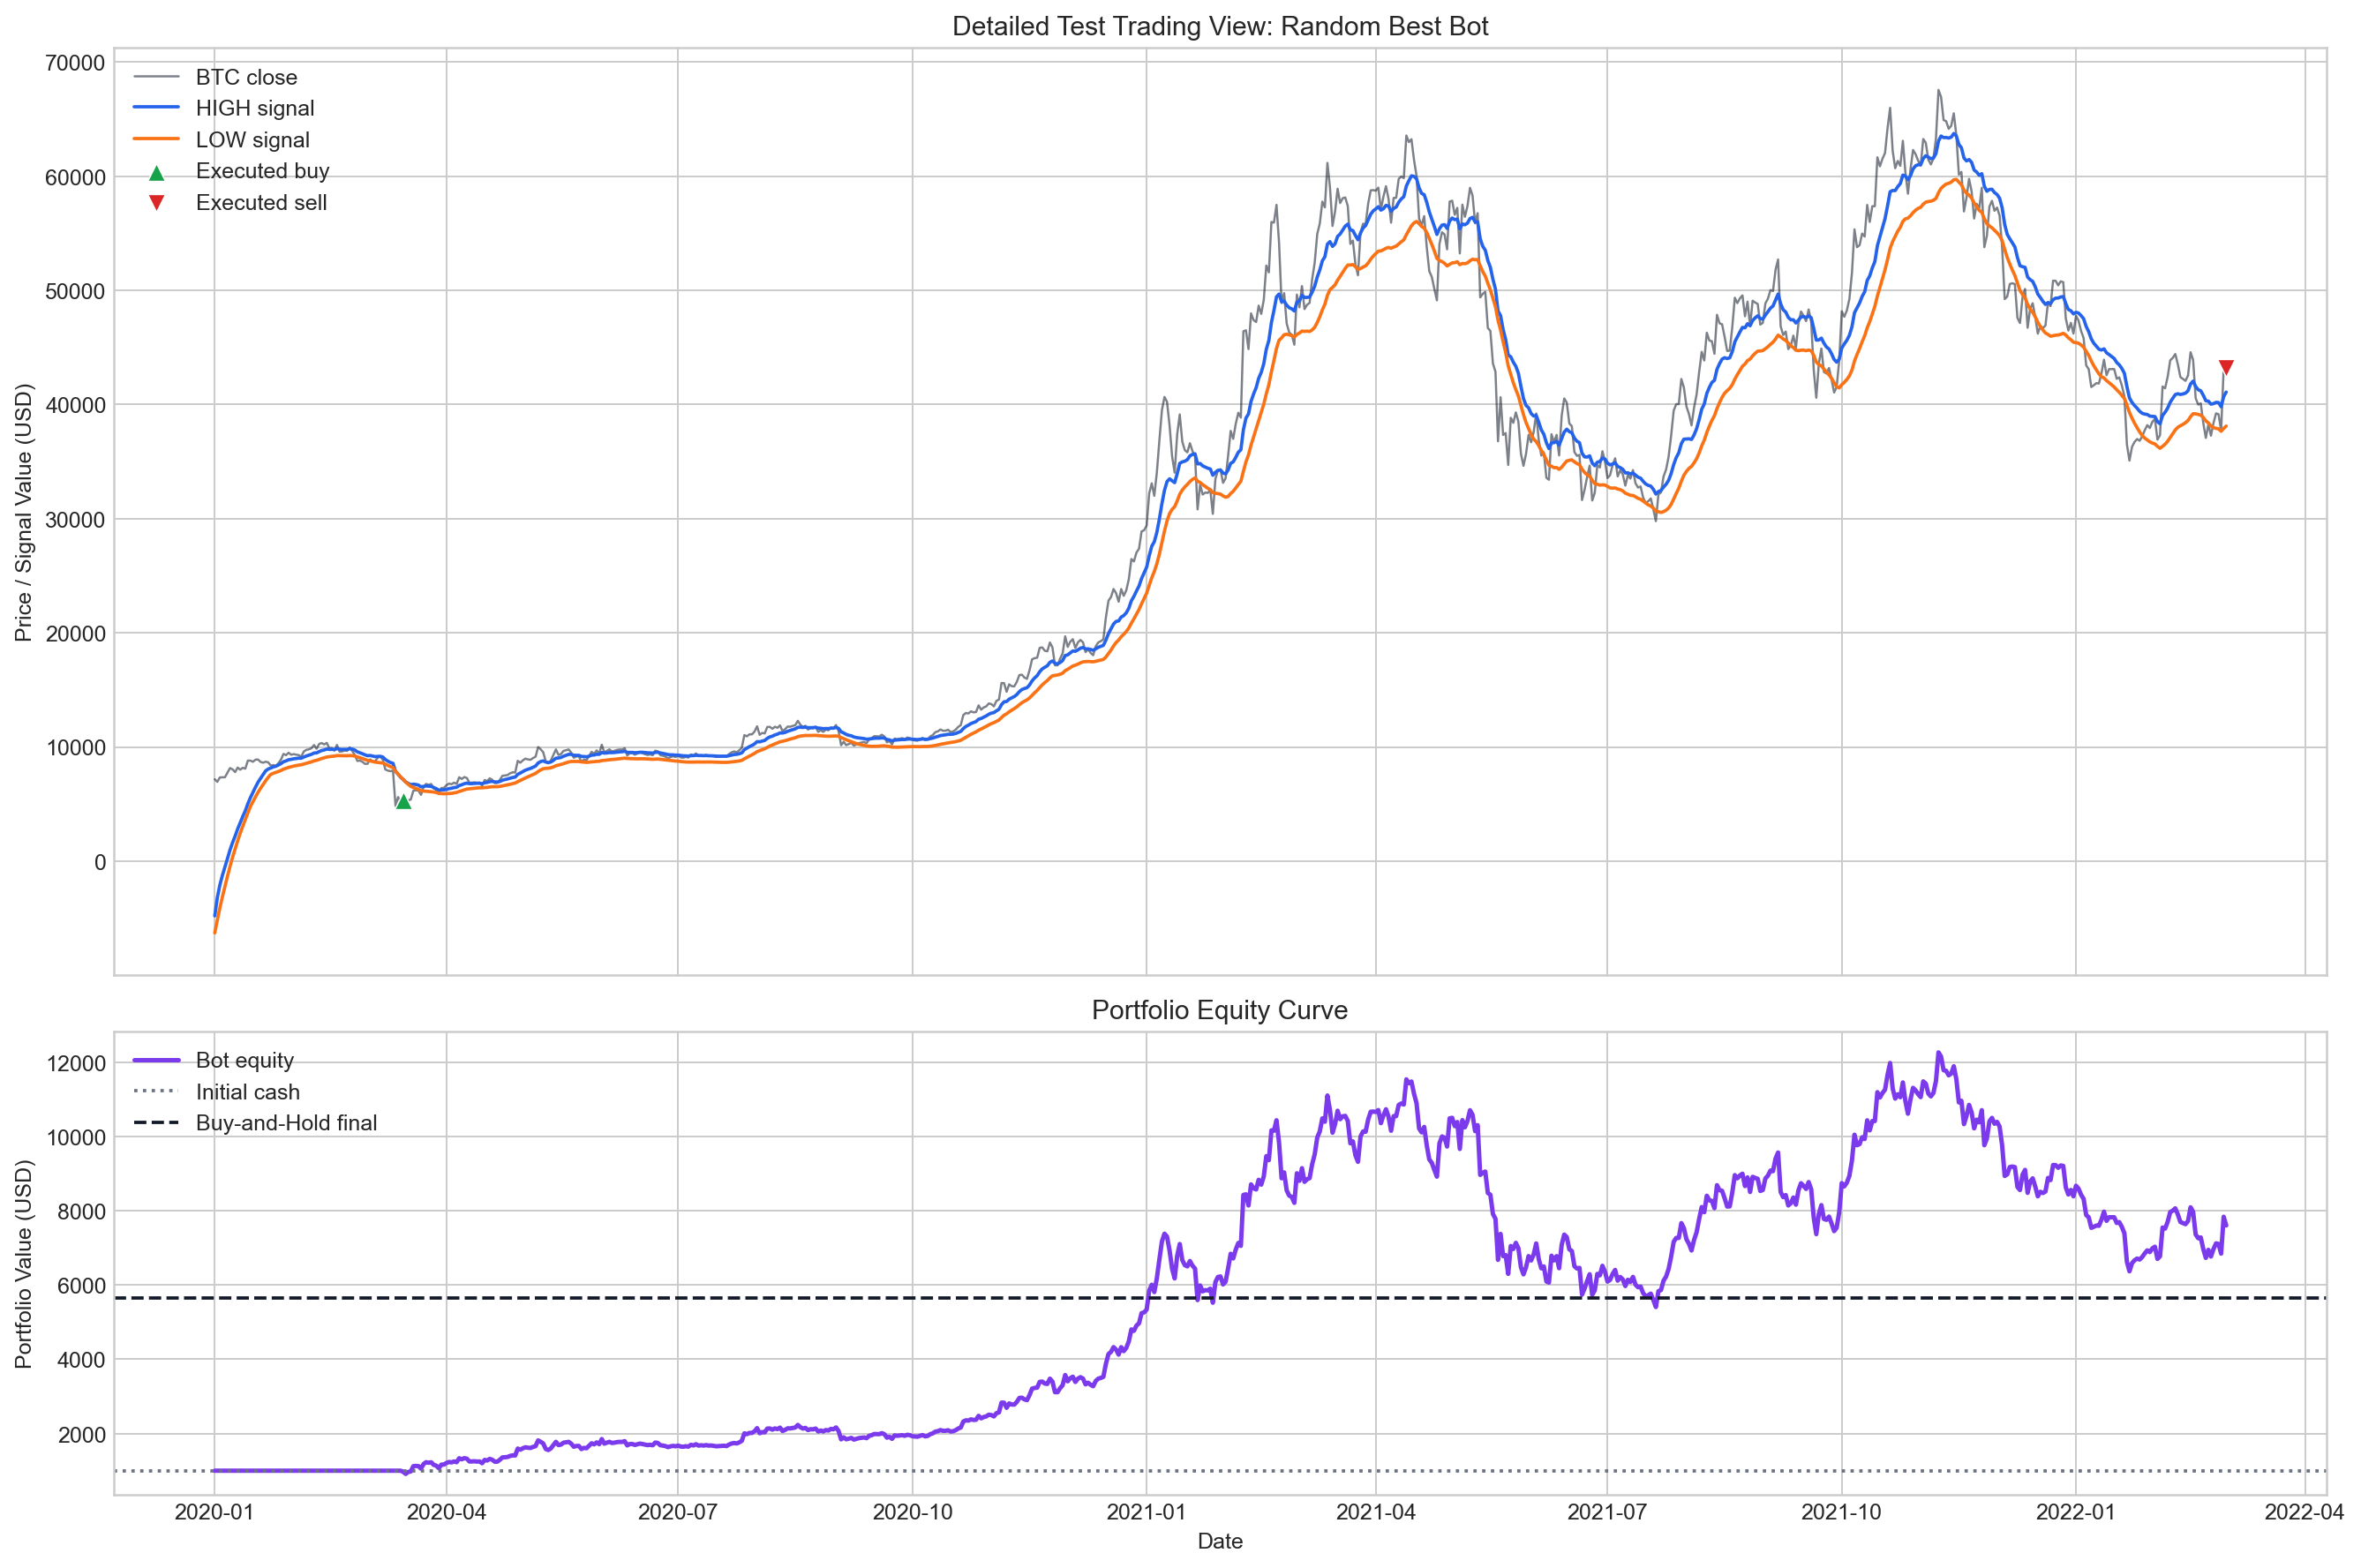
\includegraphics[width=0.92\linewidth]{outputs/figures/best_overall_trading_detail.png}
\caption{Detailed trading behaviour of the best test bot.}
\label{fig:trade}
\end{figure}

\subsection{Focus Question 2: Filter Weights, Windows, and Signal Structure}

The interpretability of the 14-dimensional bot stems from the weights and window lengths of the SMA, LMA, and EMA in the HIGH/LOW signals. Figure \ref{fig:weights} shows that the best test solutions found by different algorithms do not follow a uniform weighting template: some HIGH signals favor the faster-responding EMA or shorter windows, while some LOW signals use longer windows to form trend baselines. This aligns with the intuition of technical analysis, namely that HIGH signals should be more sensitive and LOW signals should be smoother; however, different algorithms implement this structure in different ways.


\begin{figure}[H]
\centering
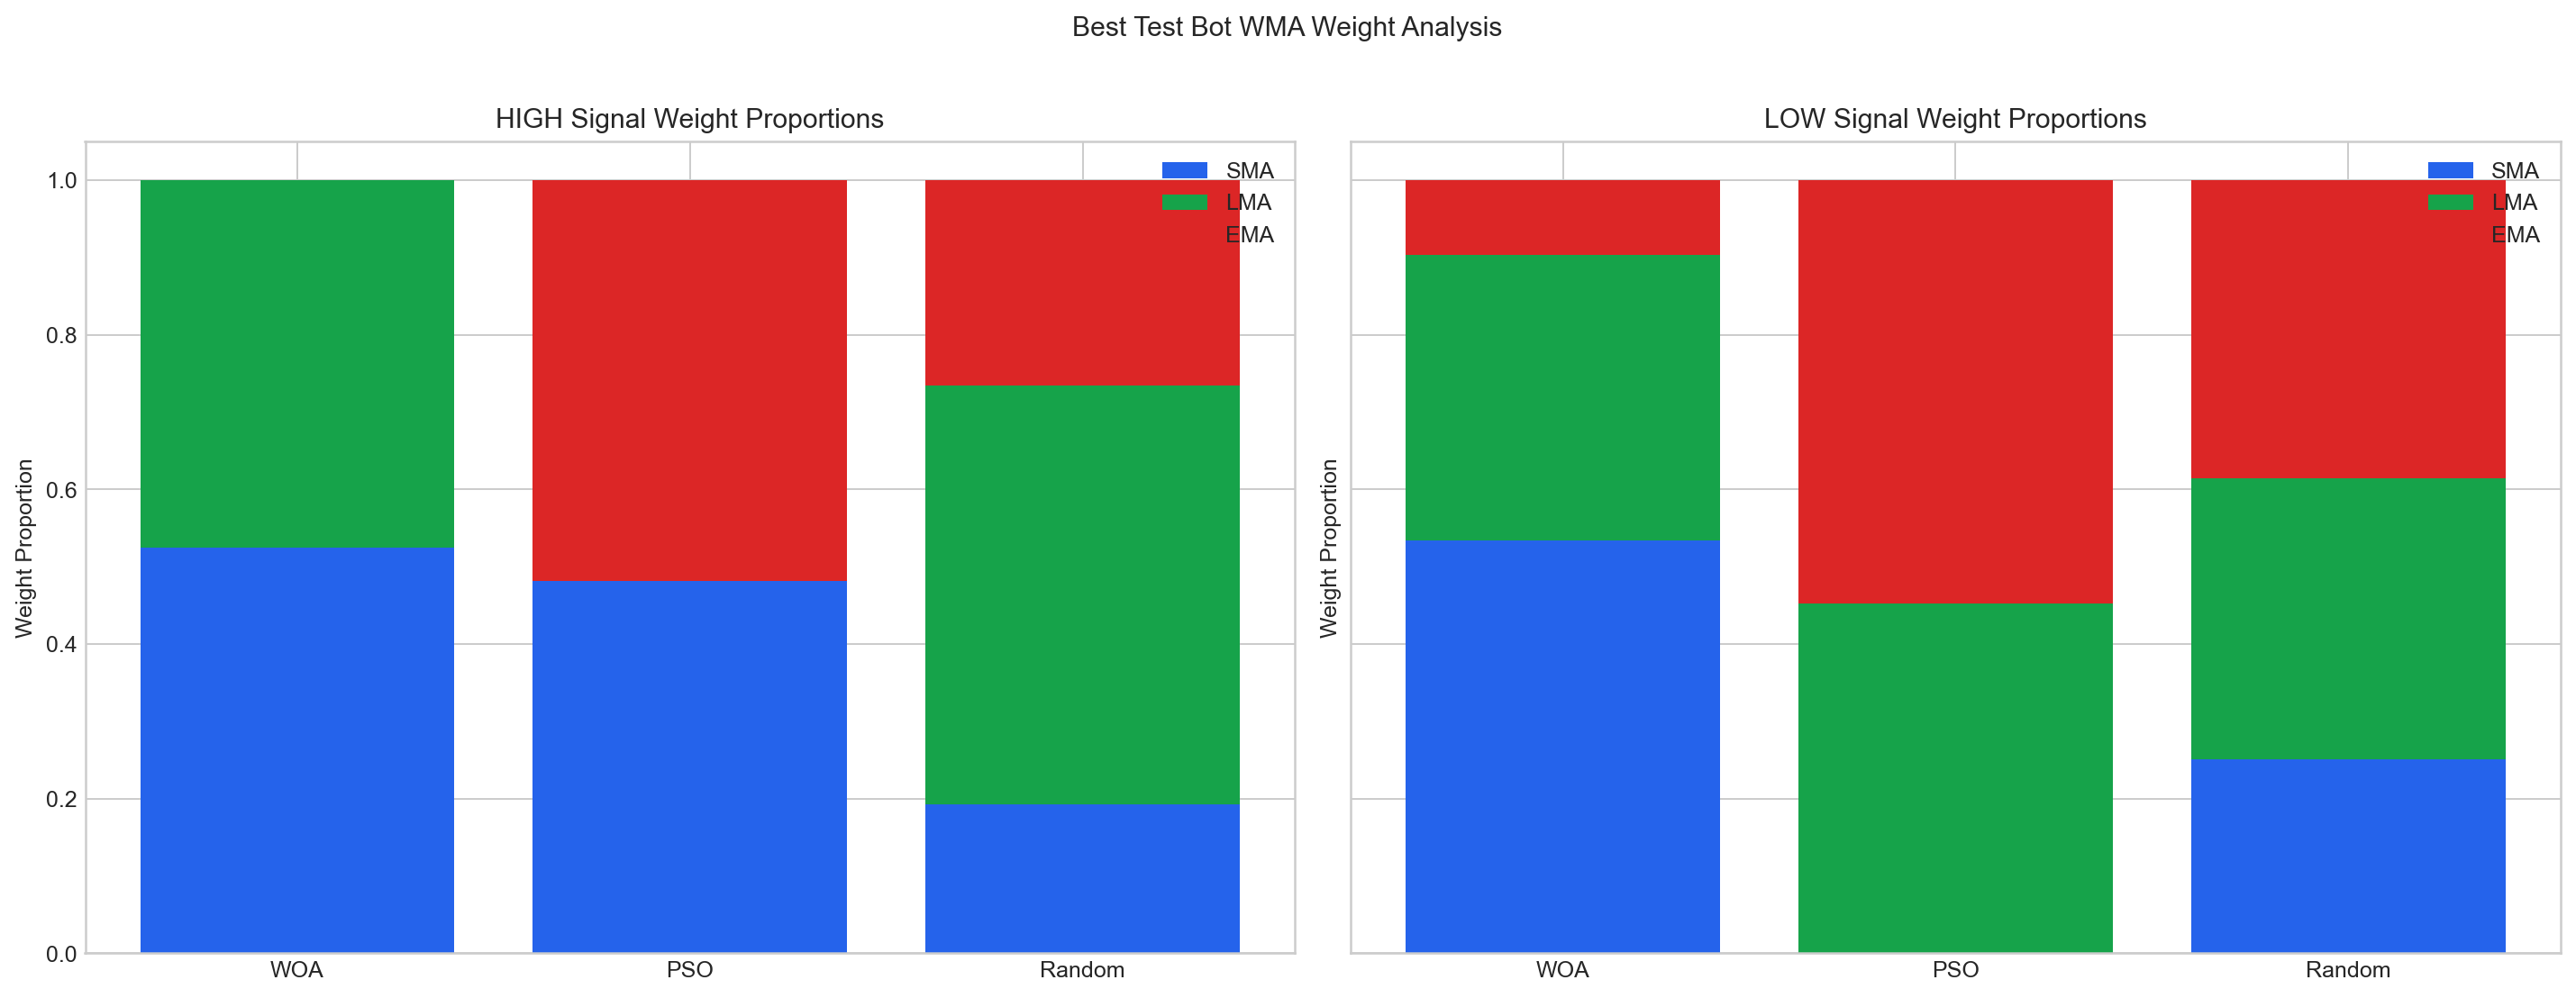
\includegraphics[width=0.88\linewidth]{outputs/figures/parameter_weight_analysis.png}
\caption{SMA/LMA/EMA weight proportions in best test solutions.}
\label{fig:weights}
\end{figure}

\begin{figure}[H]
\centering
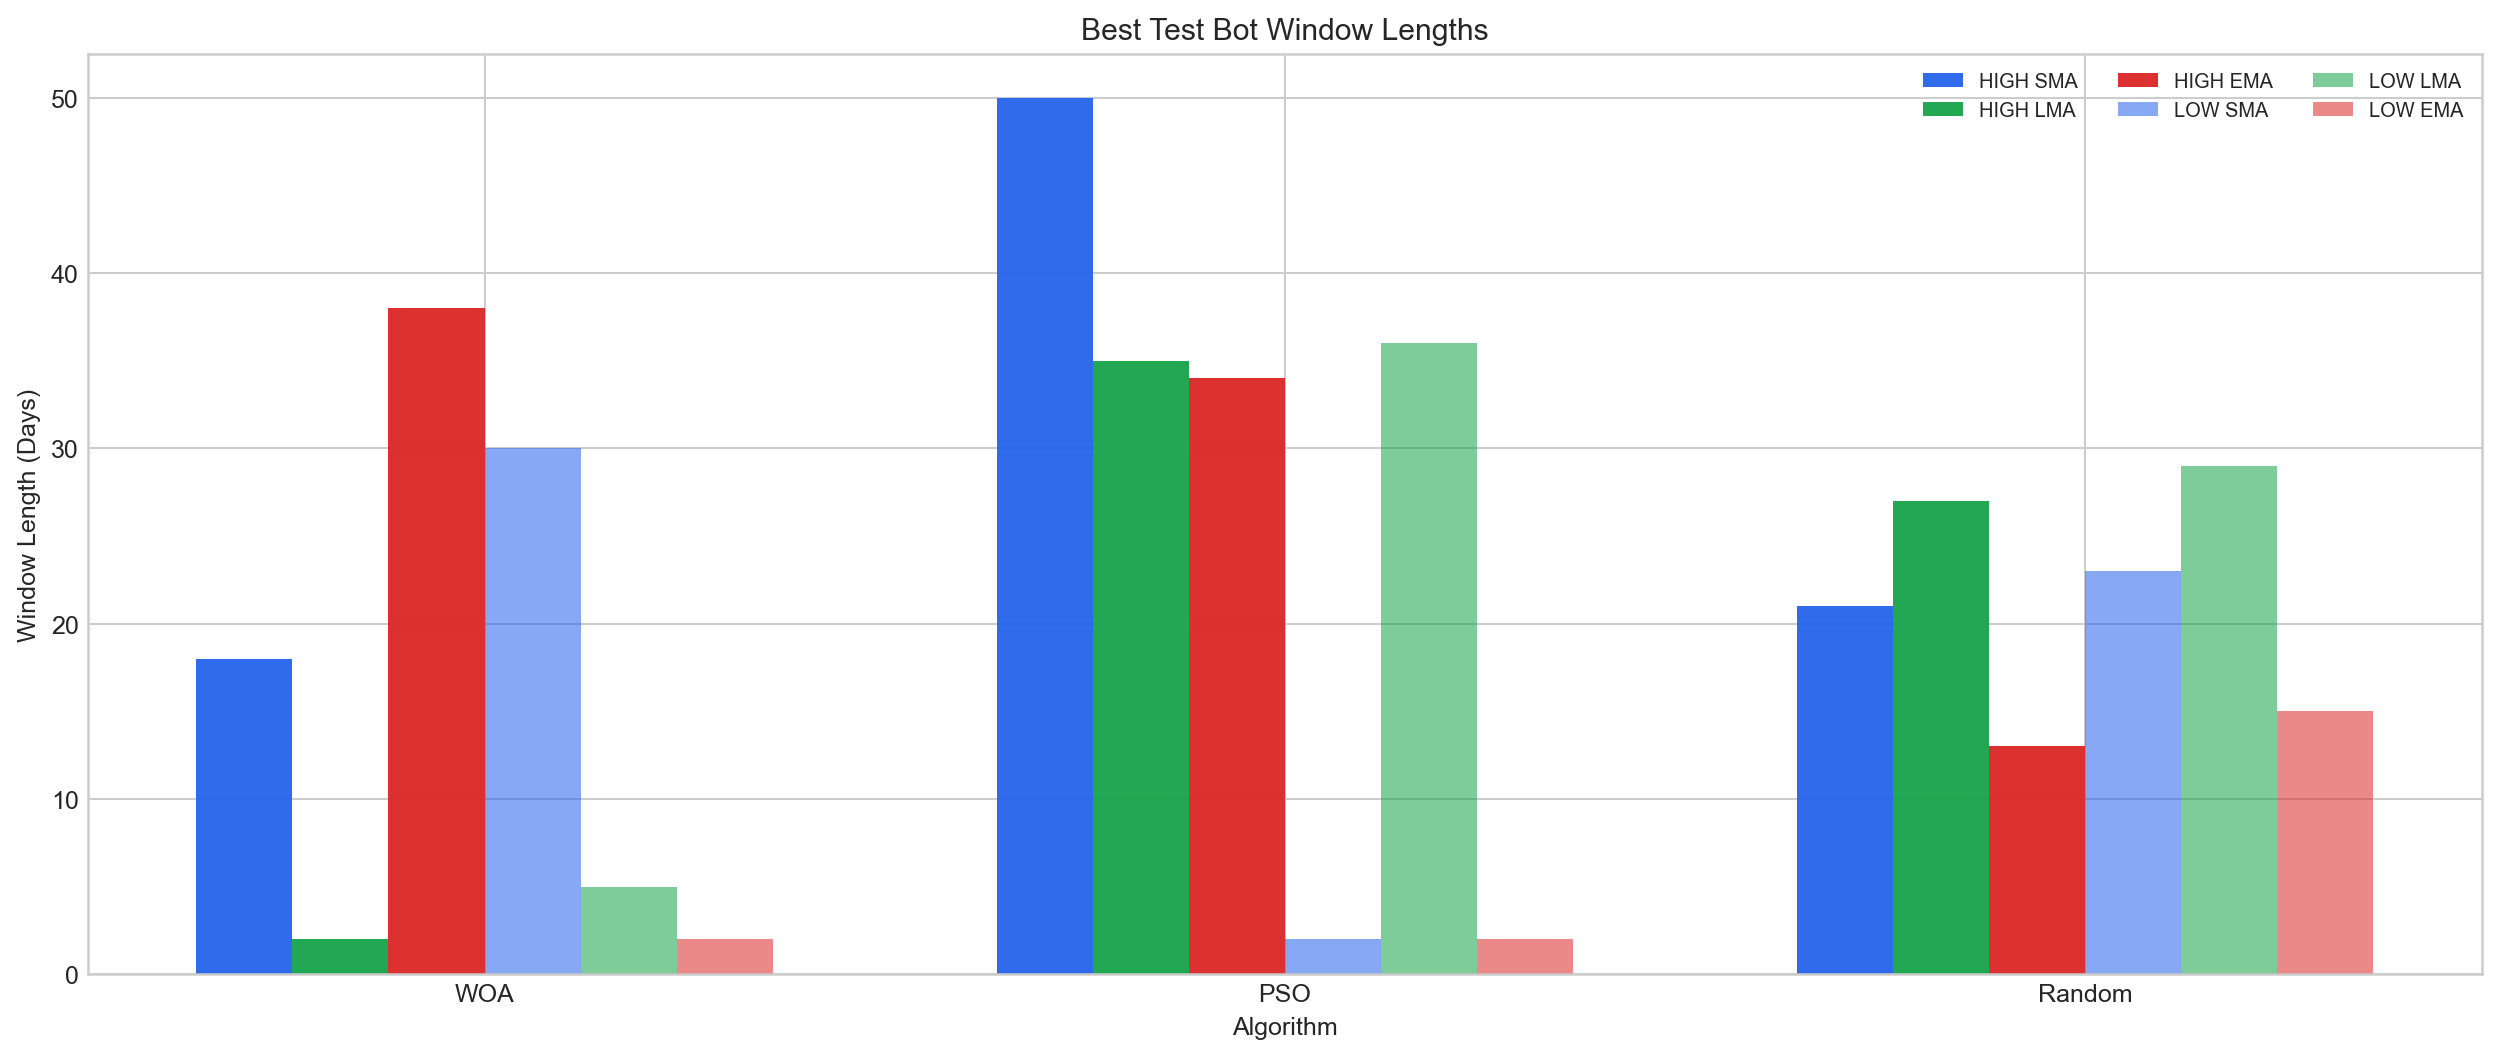
\includegraphics[width=0.88\linewidth]{outputs/figures/parameter_window_analysis.png}
\caption{Window lengths used by best test solutions.}
\label{fig:windows}
\end{figure}

These parameter analyses should not be interpreted as ablation experiments comparing the SMA, LMA, and EMA filters in isolation; rather, they illustrate how the optimization algorithm allocates filter weights and window lengths within a composite signal space. Since the structures of the best test solutions are not consistent, relying solely on the optimal parameters from the training set to assess the effectiveness of the strategy is unreliable. A more reasonable conclusion is that composite filters offer richer signal representation capabilities, but their ultimate performance still depends on whether they can maintain stability during the unseen test period.

\subsection{Focus Question 3: Dimensionality and Search-Space Trade-Offs}

Figure \ref{fig:dimension} compares the 14-dimensional Composite Bot with the 2-dimensional Simple Bot. The 2-dimensional Simple Bot still achieves approximately 40,000 USD on the training set, but its test set mean is only 600--700 USD, which is below the initial capital. The 14-dimensional Bot performs significantly better on the test set, indicating that a richer combination of filters and window parameters does indeed provide greater expressive power; however, it still does not consistently outperform Buy-and-Hold, suggesting that a higher-dimensional space does not automatically solve the generalization problem.

\begin{figure}[H]
\centering
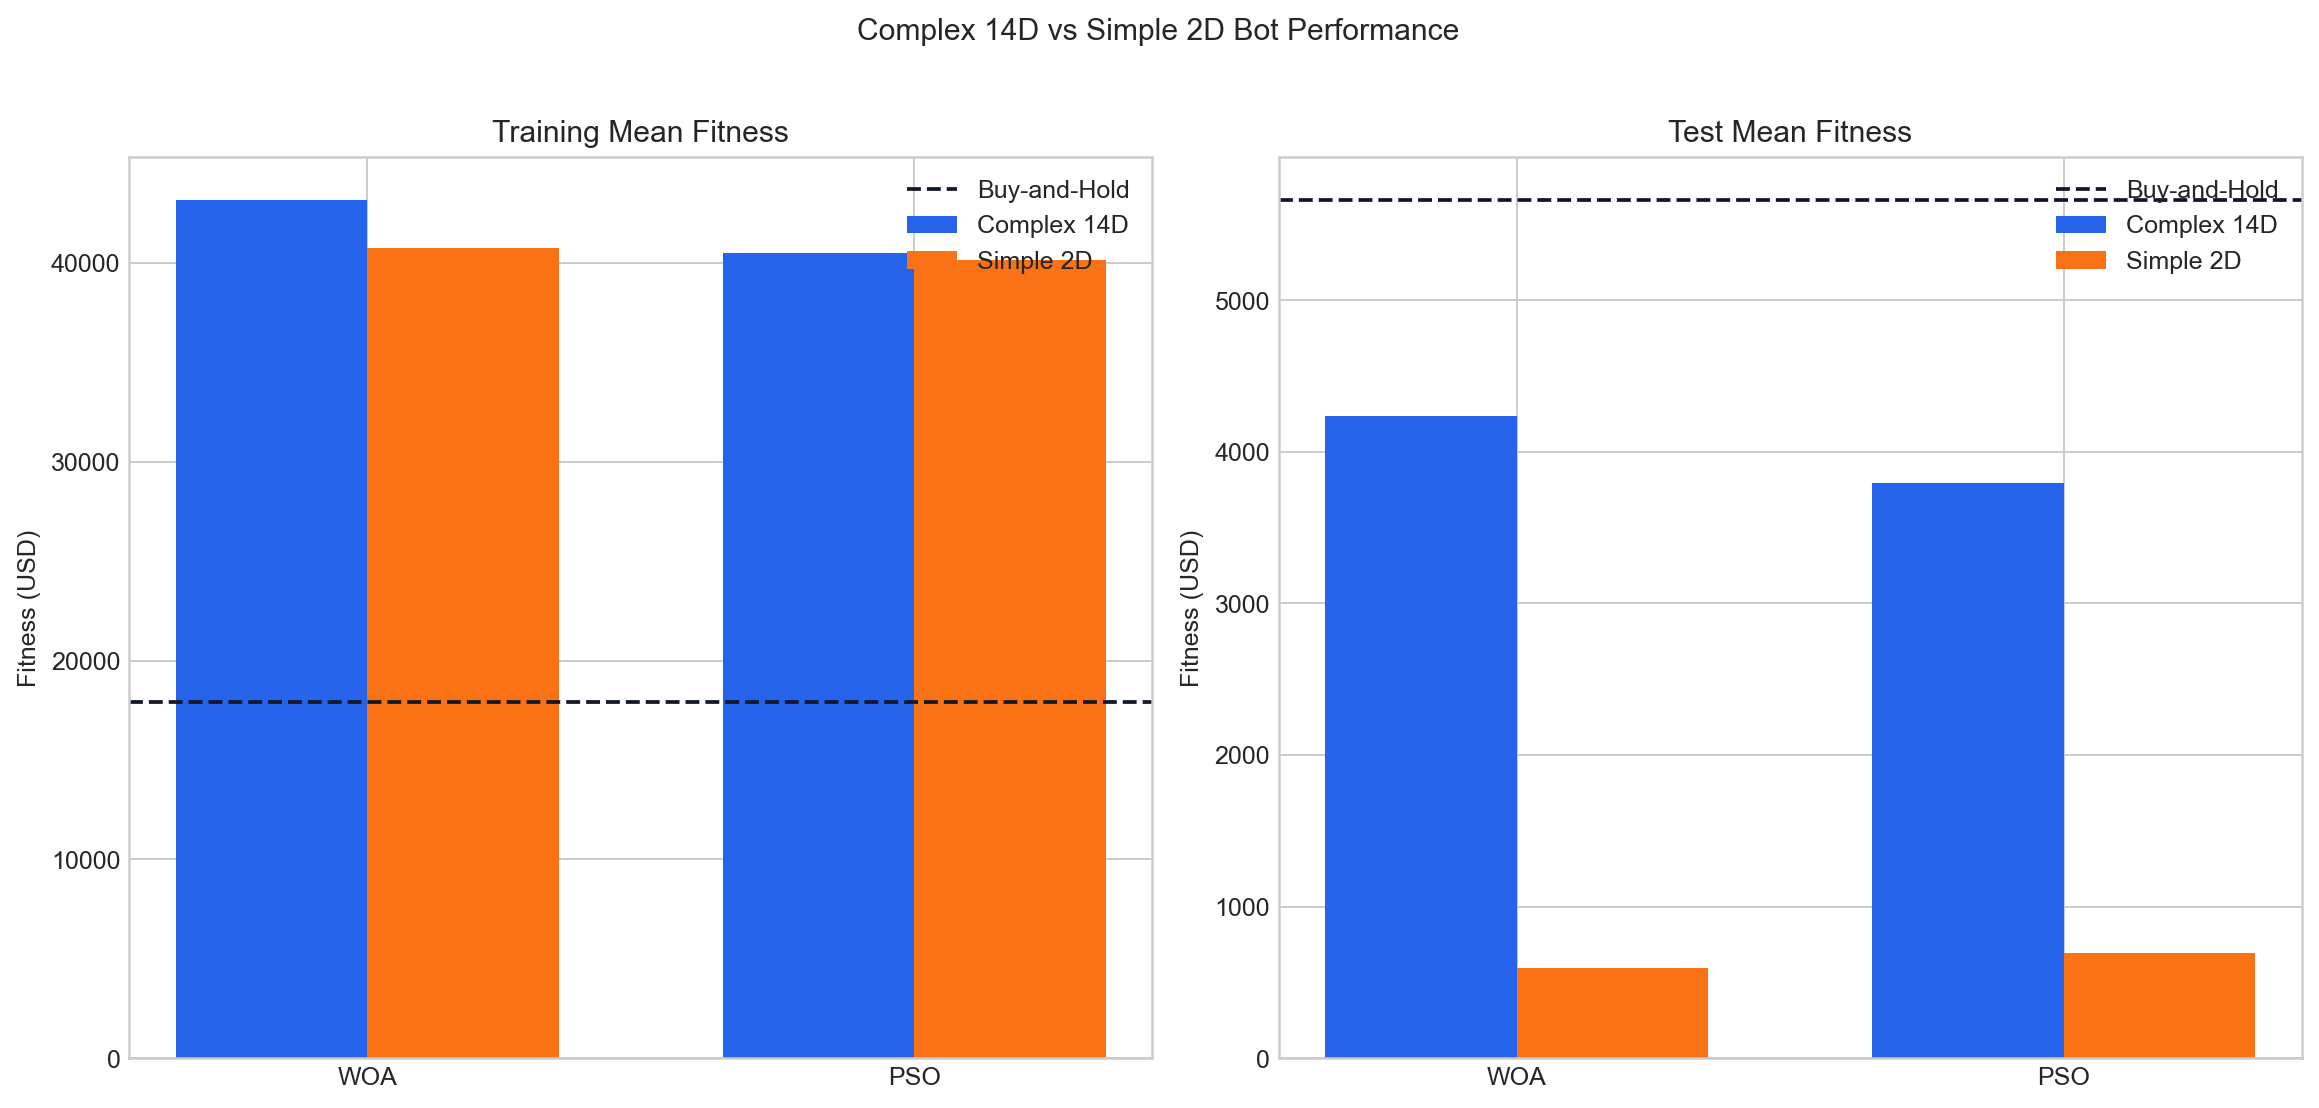
\includegraphics[width=0.86\linewidth]{outputs/figures/dimension_comparison.png}
\caption{Complex 14D bot versus Simple 2D bot.}
\label{fig:dimension}
\end{figure}

PSO population sensitivity further illustrates the trade-offs in search budgets. Figure \ref{fig:pso-sensitivity} shows only the best-so-far convergence on the training set: with a population size of 20, there are approximately 250 updates under a fixed budget, resulting in the fastest improvement on the training set; with a population size of 100, there are only about 50 updates, leading to a broader exploration but less refinement. This training curve does not directly represent generalization ability; therefore, it must be analyzed in conjunction with the unseen test performance shown in Figure \ref{fig:pso-test}.

\begin{figure}[H]
\centering
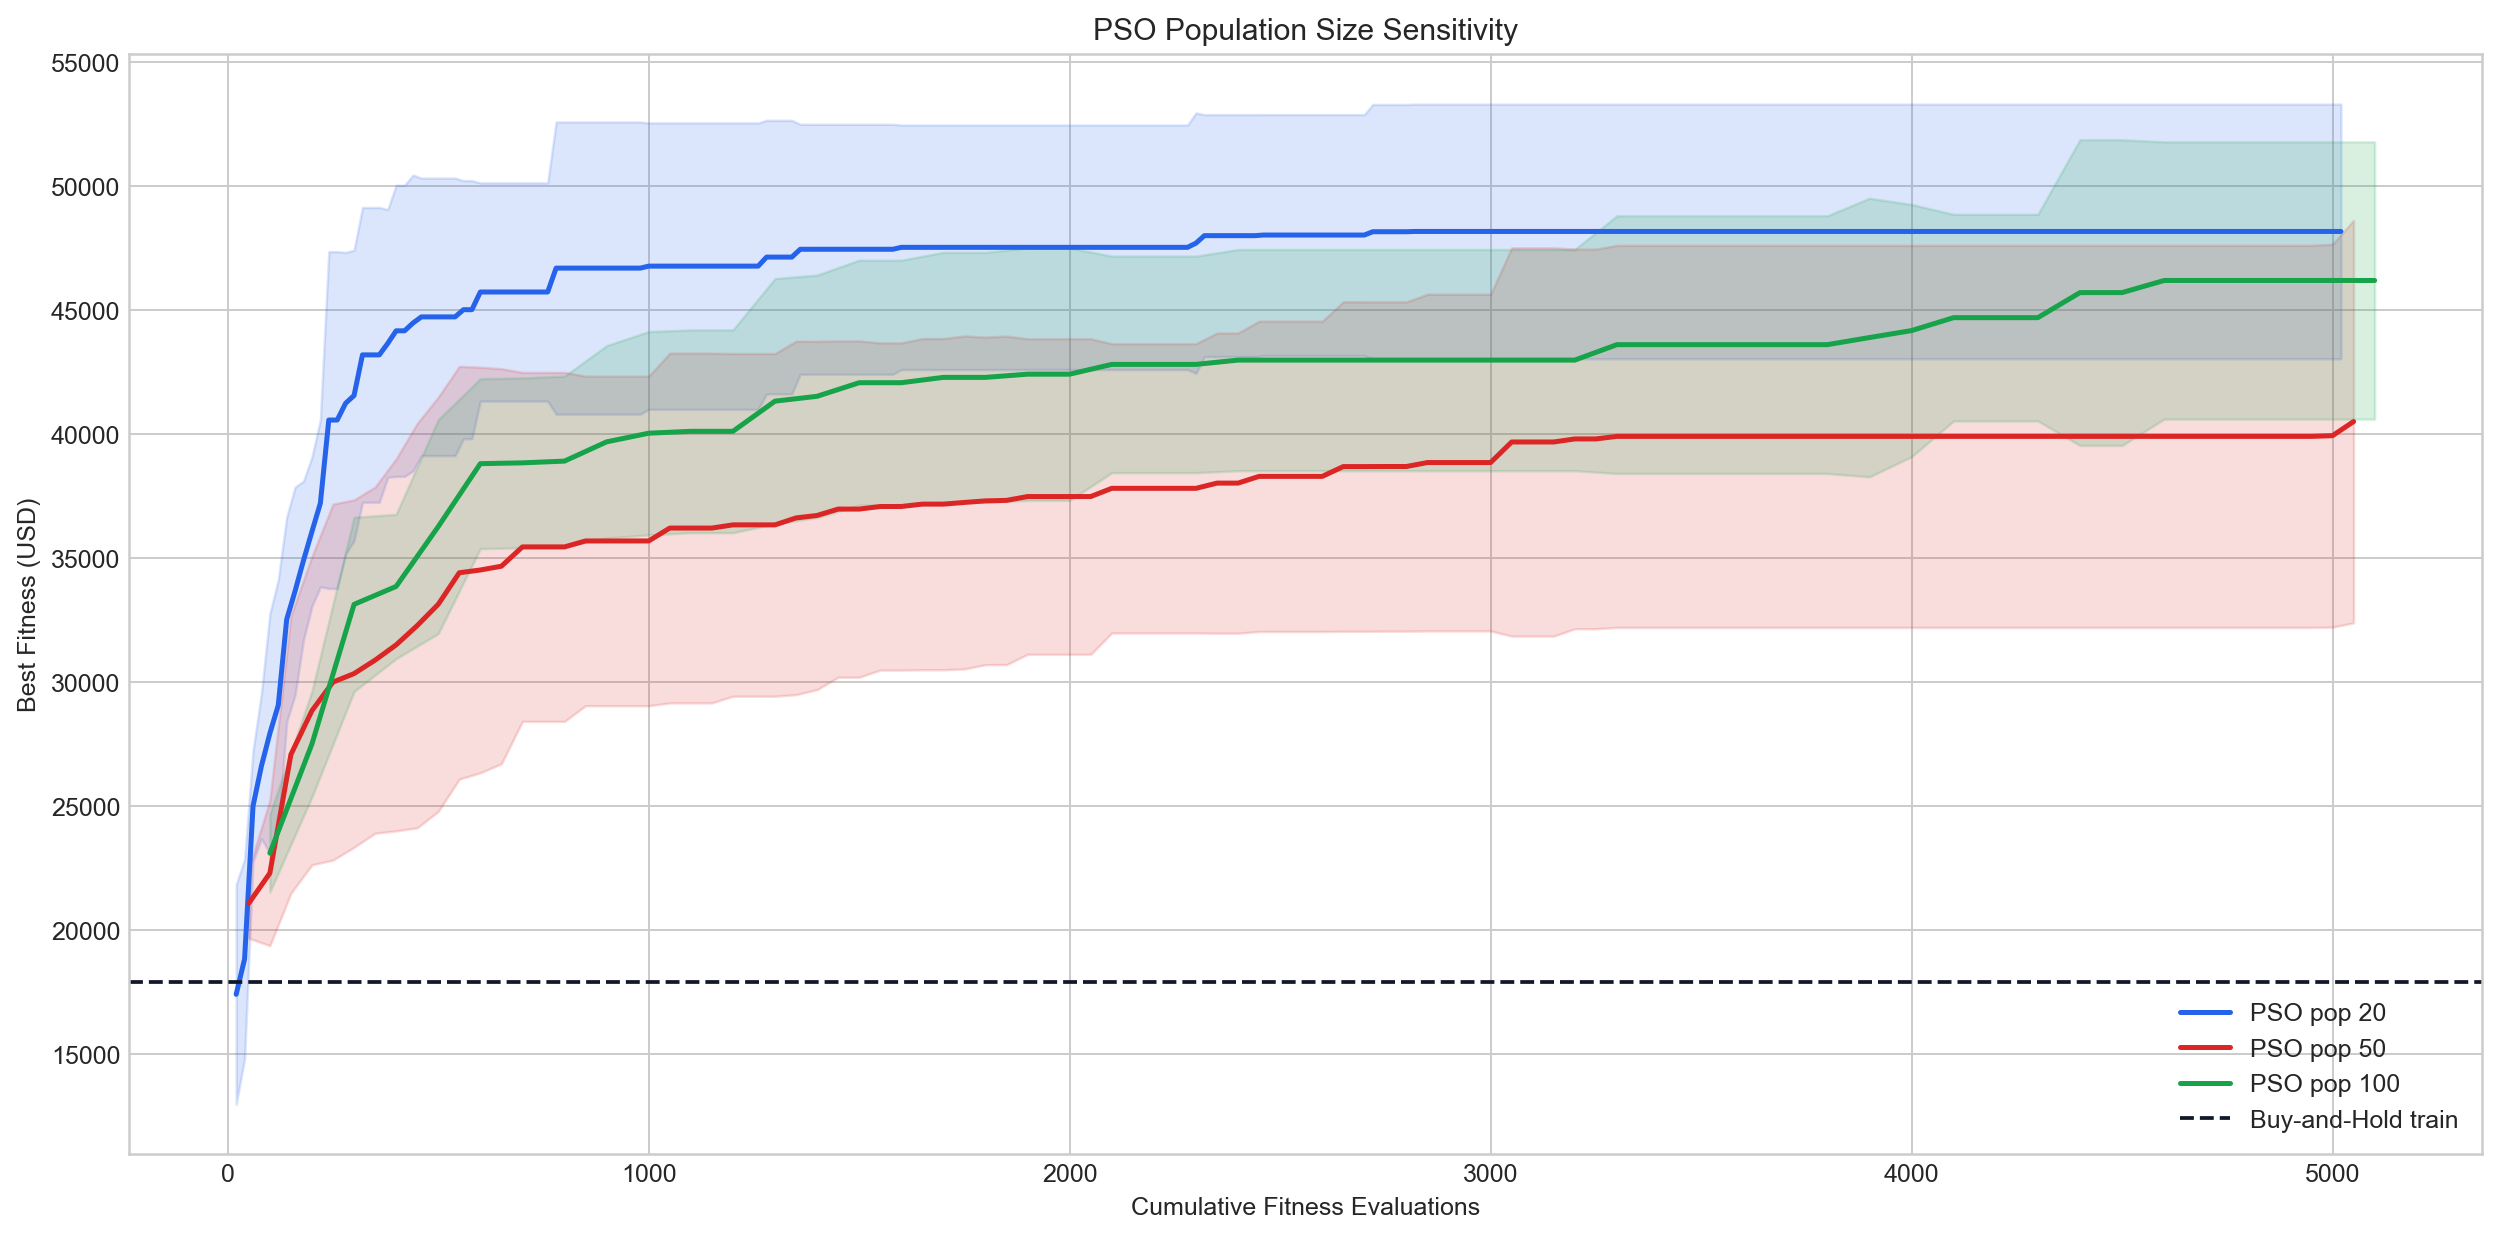
\includegraphics[width=0.88\linewidth]{outputs/figures/pso_population_sensitivity.png}
\caption{PSO population-size training convergence under fixed evaluation budget.}
\label{fig:pso-sensitivity}
\end{figure}

\begin{figure}[H]
\centering
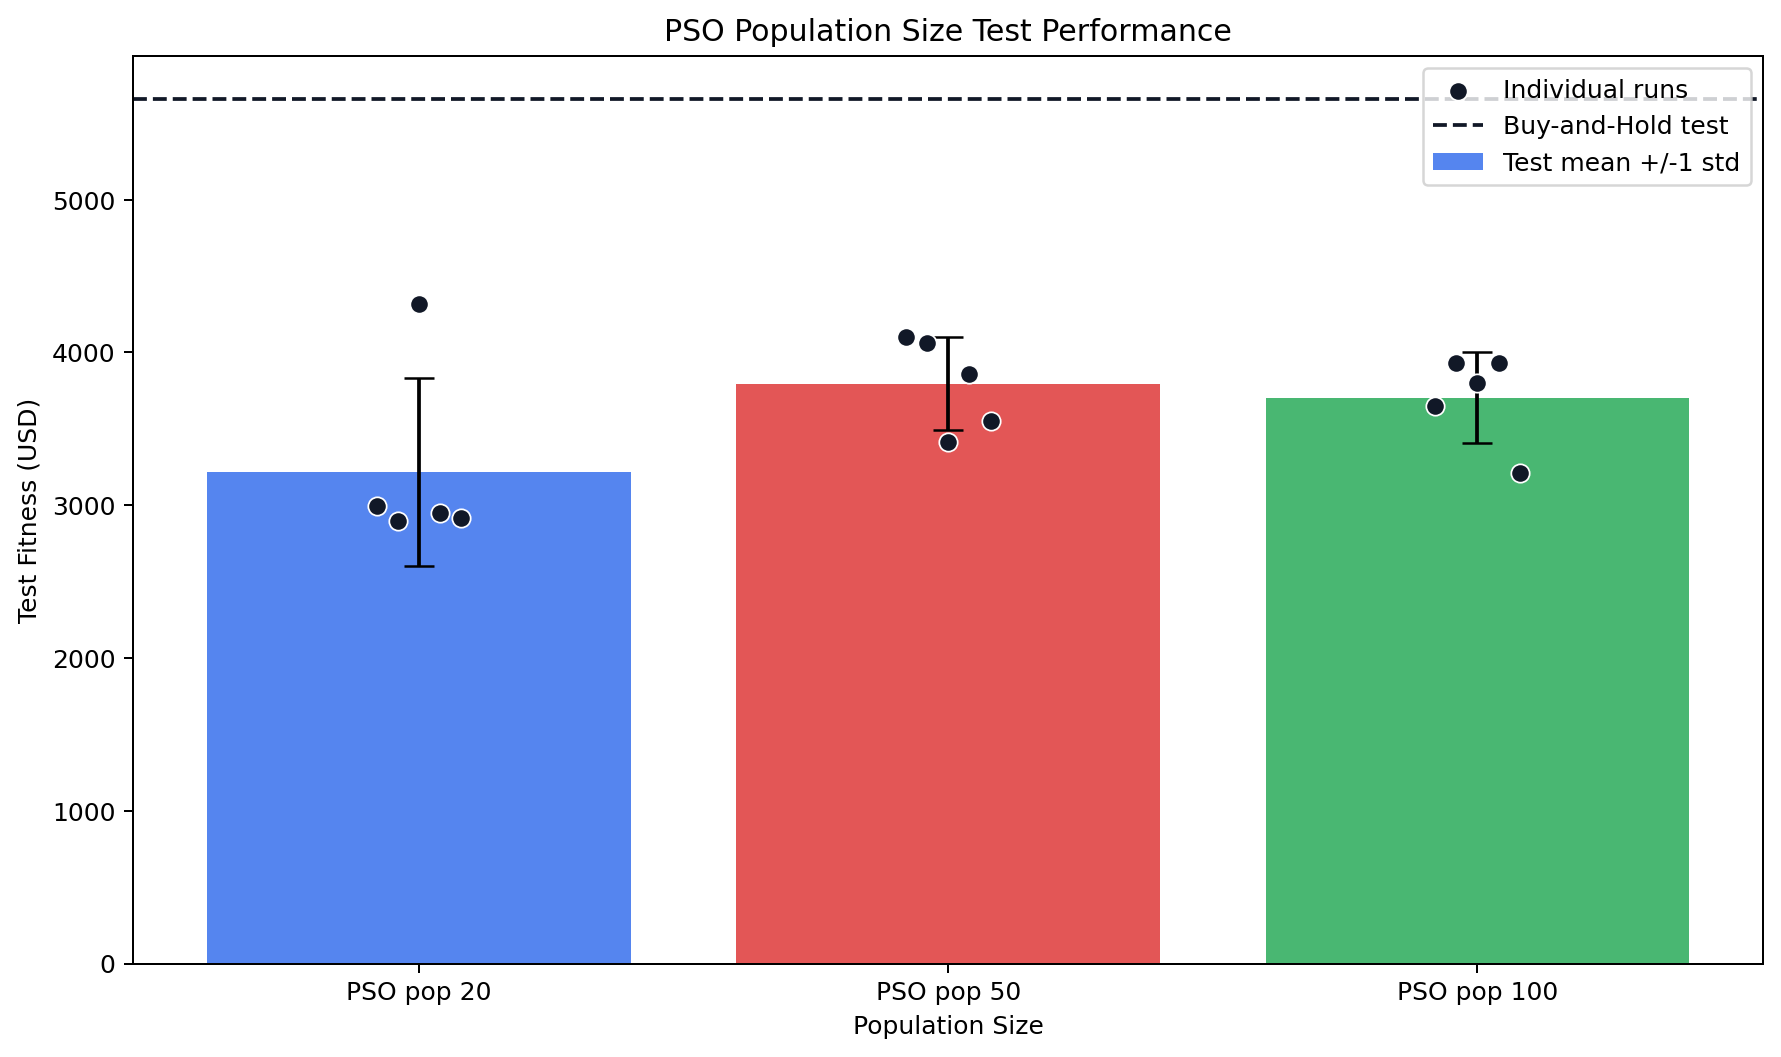
\includegraphics[width=0.78\linewidth]{outputs/figures/pso_population_test_performance.png}
\caption{PSO population-size final test performance.}
\label{fig:pso-test}
\end{figure}

Figure \ref{fig:pso-test} shows that while a population size of 20 yields the highest mean on the training set, it yields the lowest mean on the test set, suggesting that the increased number of iterations in smaller populations may have led to a stronger reliance on local patterns during the training phase. Population size 50 yields the highest test mean, demonstrating a more balanced exploration/refinement trade-off; the test performance of population size 100 is similar but slightly lower, possibly because each particle receives an insufficient number of update rounds within the fixed evaluation budget.


\section{Discussion and Conclusions}

Regarding the first focus question, both WOA and PSO were more effective than Random Search at improving the training set fitness within the same budget, with WOA outperforming PSO in terms of average train/test performance; however, the test averages for both methods remained lower than those of Buy-and-Hold. Regarding the second focus question, the weights and window lengths of SMA, LMA, and EMA endow the 14-dimensional Bot with greater expressive power and make the trading signals easier to interpret; however, the parameter structures of the different best test solutions vary significantly, indicating that there is no stable, fixed template. Regarding the third focus question, the 14-dimensional Bot significantly outperforms the 2-dimensional Simple Bot in test performance; however, the larger search space still poses a risk of overfitting, requiring an appropriate budget and a robust fitness design.

The most important conclusion of this project is that historical backtest optimization does not equate to a generalizable trading strategy. In the future, rolling windows or average fitness calculated by year could be used to reduce reliance on a single training period, and a trade frequency penalty could be introduced to mitigate the impact of the 3\% fee. Overall, the value of WOA/PSO lies in demonstrating how to search complex parameter spaces, while the Random Search and Buy-and-Hold baselines remind us that generalization ability is more important than the highest return on the training set.

\begin{thebibliography}{9}
    
\bibitem{mirjalili2016}
S. Mirjalili and A. Lewis, ``The Whale Optimization Algorithm,'' \textit{Advances in Engineering Software (1992)}, vol. 95, pp. 51--67, May 2016, doi: 10.1016/j.advengsoft.2016.01.008.

\bibitem{kennedy1995}
J. Kennedy and R. Eberhart, ``Particle swarm optimization,'' in \textit{1995 IEEE International Conference on Neural Networks Proceedings}, IEEE, 1995, pp. 1942--1948 vol. 4, doi: 10.1109/ICNN.1995.488968.

\bibitem{btc_dataset}
P. Kottarathil, ``Bitcoin Historical Dataset,'' Kaggle. Accessed: May 22, 2026. [Online]. Available: \url{https://www.kaggle.com/datasets/prasoonkottarathil/btcinusd}

\end{thebibliography}

\end{document}
